\section{Experimental Evaluation}

This section provides a comprehensive analysis of the methodologies employed in this study. It commences with a detailed description of the datasets and metrics (Section~\ref{sec: dataset_and_metrics}). Subsequently, Section~\ref{sec: experiments} presents an extensive experimental evaluation, encompassing an analysis of instance mask formulation, comparisons of various attention mechanisms, an examination of auxiliary one-to-many set prediction loss, an efficiency analysis of the proposed Bezier deformable attention, and a study on multi-modal fusion involving camera, radar, lidar, and SDMap. The results are juxtaposed with state-of-the-art methods on both OpenLane-V1 and OpenLane-V2.

Supplementary material provides additional details on the various loss functions (Section~\ref{sup_sec: experiments_loss_functions}), the implementation specifics of the training setup, dataset preprocessing and the proposed architecture (Section~\ref{sup_sec: implementation_details}), and further experiments (Section~\ref{sup_sec: experiments}) including view transformation, backbone variations, number of epochs, number of encoder and decoder layers, and efficient multi-scale implementation ablations.


\subsection{Dataset and Metrics}
\label{sec: dataset_and_metrics}

\subsubsection{Datasets}

\begin{figure}[tb]
  \centering
  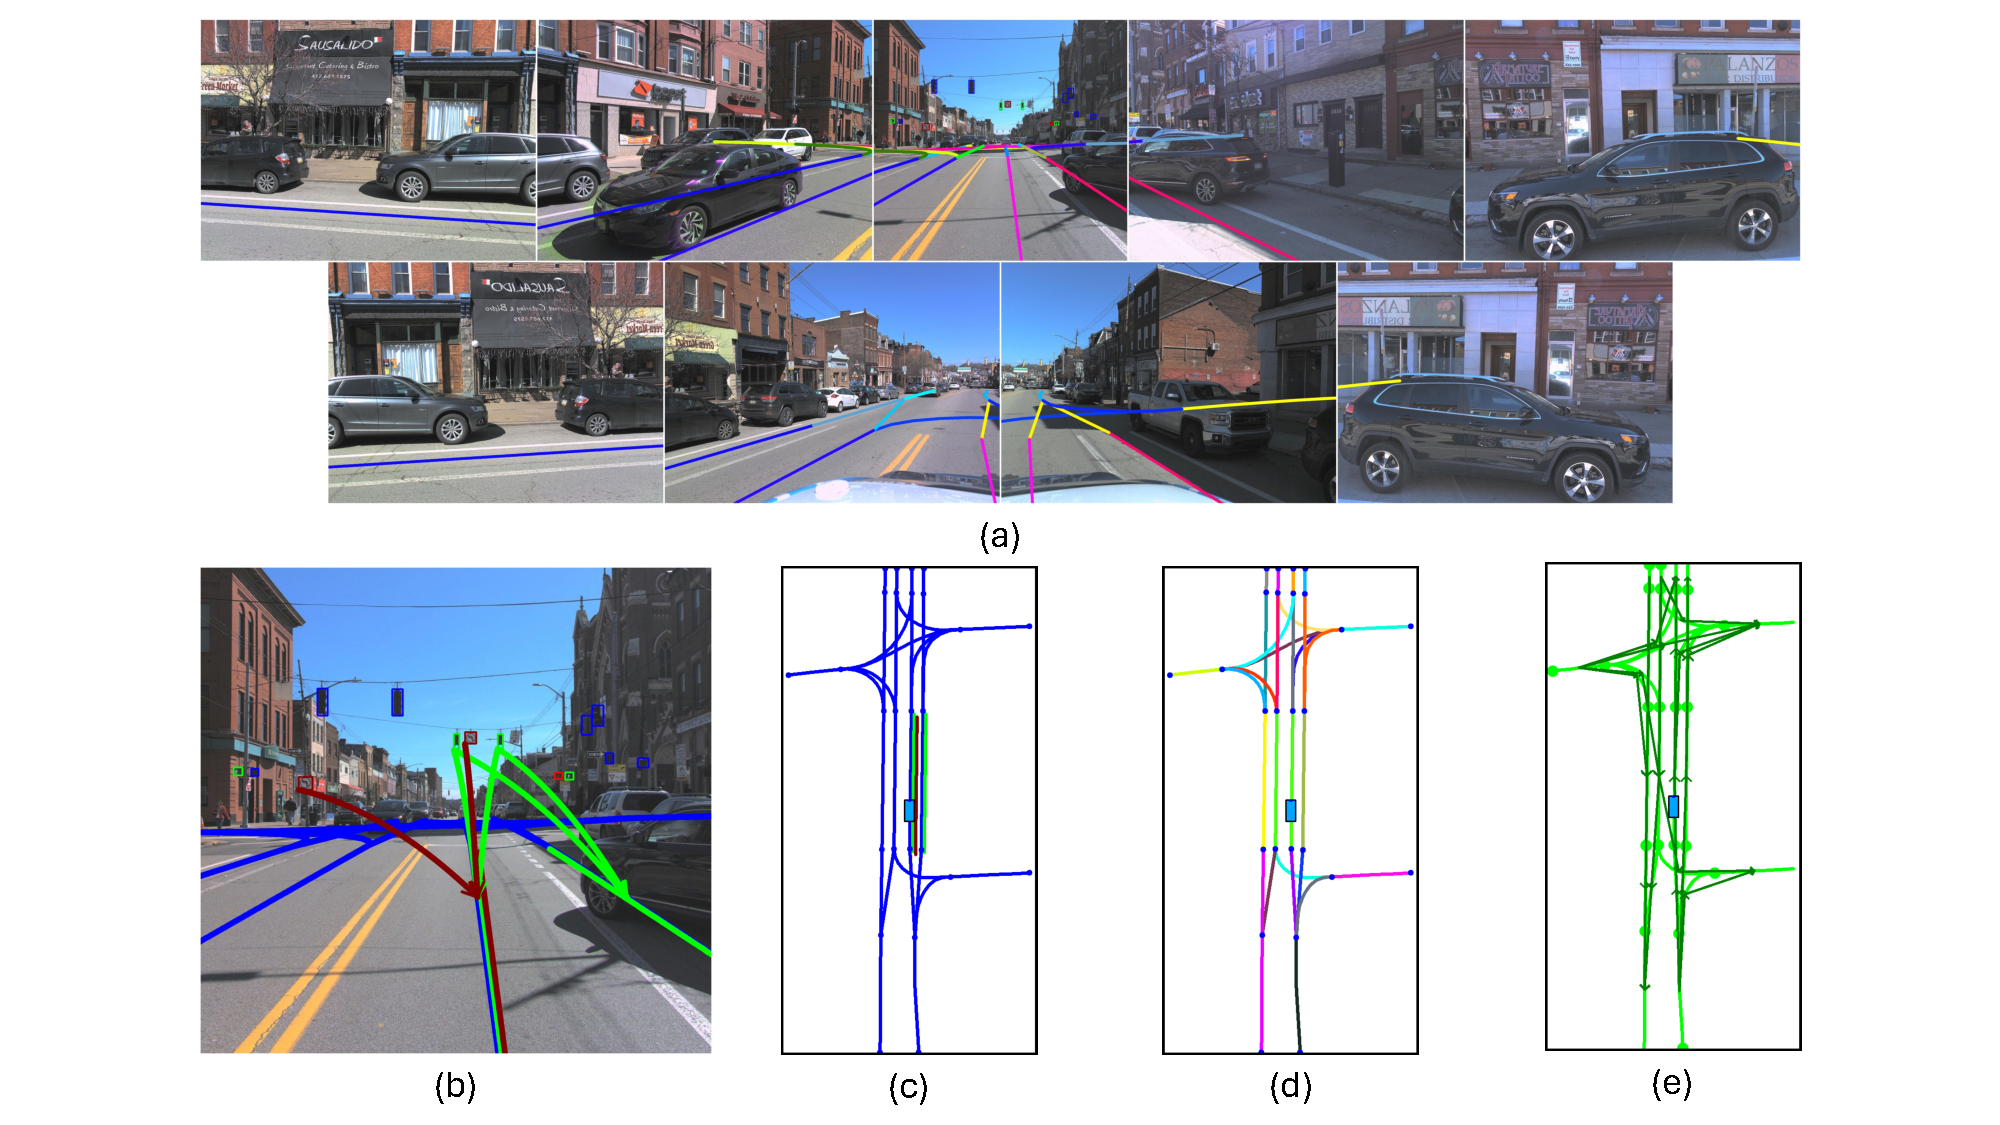
\includegraphics[width=\linewidth]{dataset.pdf}
  \caption{Perspective-view (PV) and bird’s-eye-view (BEV) samples from the OpenLane-V2 dataset. (a) and (d) show centerline instances in PV and BEV domains, respectively, with each color representing a distinct instance. (b) and (c) illustrate centerlines with colors indicating topological relationships between centerlines and traffic elements in PV and BEV. (e) visualizes the topological relationships among different centerlines, where directed arrows indicate connectivity between centerlines.}
  \label{fig: dataset_figure}
\end{figure}

The OpenLane-V2 dataset \cite{wang2024openlane} is a centerline detection and road topology understanding dataset and has two subsets: Subset-A and Subset-B. Subset-A is derived from the Argoverse 2 (AV2) \cite{wilson2023argoverse} dataset, containing samples from six cities (e.g., Miami, Pittsburgh, Austin), collected using a seven-camera setup with the front camera positioned vertically. This subset contains 22,477 training samples, 4,806 validation samples, and 4,816 test samples, all with a resolution of $2048\times1550$ pixels. Multi-modal fusion studies are conducted with lidar data and SDMap, and no radar data is available in Subset-A.

Subset-B is based on the NuScenes \cite{caesar2020nuscenes} dataset and contains data collected from Boston and Singapore, using a six-camera setup. It includes 27,968 training, 6,019 validation, and 6,008 test samples, with an image resolution of $1600\times900$ pixels. Subset-B has a higher proportion of night and rainy scenes compared to Subset-A, but lacks ground height information. Sensor fusion studies are implemented with both radar and lidar data, but no available SDMap information in this subset. The details of the image pre-processing pipeline for both subsets are provided in Supplementary Section \ref{sup_sec: dataset_preprocessing}.

Figure \ref{fig: dataset_figure} presents PV and BEV images from a random sample in Subset-A of the OpenLane-V2 dataset. Due to the vertical positioning of the camera, the front view in the PV domain is cropped. As shown in subfigures (a) and (d), centerline instances are visualized in PV and BEV domains, respectively, with each color representing a distinct instance. Subfigures (b) and (c) highlight the topological relationships between centerlines and traffic elements using color-coded representations in both PV and BEV views. Subfigure (e) illustrates the topological relationships among different centerlines, where directed arrows indicate connectivity between them. More ground truth examples are shown in Supplementary Figure \ref{sup_fig: pv_and_bev_samples} in Section \ref{sup_sec: visual_results}. 

The OpenLane-V1 dataset  \cite{chen2022persformer} is a comprehensive benchmark for 3D lane detection, derived from the Waymo Open dataset. It consists of 1000 segments with 200K frames, captured under diverse conditions at $1920\times1280$ resolution. This dataset provides diverse and challenging scenarios for evaluating lane detection algorithms, including a wide range of weather conditions, lighting variations, and road types. 


\subsubsection{Metrics}

\sloppy
For the evaluation of centerlines and traffic elements in both Subset-A and Subset-B of OpenLane-V2, the considered area extends +50 to -50 meters forward and +25 to -25 meters sideways. Both centerline detection and traffic element recognition are evaluated using the Mean Average Precision (mAP) metric. True positive samples are identified using different distance measures depending on the task. For centerline detection, the Fréchet distance and Chamfer distance are used. The Fréchet distance accounts for both distance and directionality between predicted and ground truth centerlines, whereas the Chamfer distance only considers distance, disregarding directionality. For traffic element recognition, the Intersection over Union (IoU) metric is used with a threshold of 0.75. The Fréchet distance thresholds are 1, 2, and 3 meters, while the Chamfer distance thresholds are 0.5, 1, and 1.5 meters. The mean AP of different thresholds is denoted as $\text{DET}_{l}$ for Fréchet-based mAP and $\text{DET}_{l\_ch}$ for Chamfer-based mAP, and $\text{DET}_{t}$ for IoU-based mAP.

In addition to these metrics, a specialized mAP metric is proposed to evaluate topology reasoning in the graph domain. This metric assesses the connectivity and relationships between centerlines and traffic elements. For an edge (connectivity) to be a true positive, both vertices must be correctly detected according to the Fréchet distance for centerlines and the IoU criteria for traffic elements. The topology scores are defined as $\text{TOP}_{ll}$ for centerline topology and $\text{TOP}_{lt}$ for centerline-traffic element topology.


\begin{equation}
\label{Eq:OLS}
    \text{OLS} = \frac{1}{4} \bigg[ \text{DET}_{l} + \text{DET}_{t} + f(\text{TOP}_{ll}) + f(\text{TOP}_{lt}) \bigg].
\end{equation}

The evaluation framework uses the OpenLane-V2 Score (OLS) as the overall metric, which is calculated as the average of several task-specific metrics: Fréchet-based mAP for centerline prediction ($\text{DET}_{l}$), IoU-based mAP for traffic element prediction ($\text{DET}_{t}$), and the topological relationships metrics between centerlines and traffic elements ($\text{TOP}_{ll}$ and $\text{TOP}_{lt}$). The evaluation metric pipeline has been updated from version 1.0 to 1.1 to address previously identified issues, as outlined in the TopoMLP study \cite{wu2023topomlp}.

The potential shortcomings of the 1.1 baseline are discussed in the TopoMaskV2 study \cite{kalfaoglu2024topomaskv2}, and a modified baseline is proposed, which is referred to as version 1.1m in this study. While the metric itself remains unchanged, the topology scores are re-mapped such that $P(x) + 1 \times [P(x) > 0.05]$, where $P(x)$ represents the topology score. To ensure fair comparison with existing literature, state-of-the-art comparisons are conducted using V1.1, while all our ablations and hyperparameter evaluations are performed using the V1.1m baseline.


\begin{equation}
\label{Eq: OLS_l}
    \text{OLS}_{l} = \frac{1}{3} \bigg[ \text{DET}_{l} + \text{DET}_{l\_ch} + f(\text{TOP}_{ll}) \bigg].
\end{equation}

To perform ablations focused exclusively on centerline prediction and centerline topology, we use the $\text{OLS}_{l}$ metric Eq. (\ref{Eq: OLS_l}), which excludes components associated with traffic elements. Since the architectural framework of TopoBDA is specifically designed to improve centerline prediction, it is essential to develop metrics dedicated to centerline prediction and centerline topology prediction accuracy.

For 3D lane detection evaluation in the OpenLane-V1 dataset, the F1 metric is preferred, as it calculates the harmonic mean of precision and recall. A detection is considered a true positive if at least 75\% of the compared points are within the predefined threshold of 1.5 meters or 0.5 meters from the ground truth lane dividers. The detection range for the metric is set from 3 to 103 meters in the forward direction and -10 to 10 meters in the lateral direction. A threshold of 40 meters is used to distinguish between close and far ranges, with lateral and height translation errors measured separately for these regions.


\subsection{Experimental Evaluation}
\label{sec: experiments}

In this section, the experimental results are presented. The training setup, including optimizer configurations, learning rate schedules, batch size, architectural specifications, and hyperparameter settings, is described in detail in Section~\ref{sup_sec: implementation_details} of the supplementary material. This section also includes the backbone configurations, transformer parameters, loss coefficients, and implementation details necessary for reproducibility.

The experiments are structured as follows. First, the impact of the instance-mask formulation is analyzed. This is followed by a comparative evaluation of various attention mechanisms and a conceptual analysis of the auxiliary one-to-many set prediction loss. Subsequently, the performance of sensor fusion and SDMap integration, as well as the efficiency of different attention mechanisms within decoder implementations, is assessed. Finally, the results are compared against state-of-the-art benchmarks on the OpenLane-V2 and OpenLane-V1 datasets.

The supplementary material section provides further insights into our experiments (Section \ref{sup_sec: experiments}), including a comparative analysis of view transformation methods, a comparison of standard and efficient multi-scale implementations, a further efficiency analysis of attention types, the number of encoder and decoder layers, an impact of number of control points, an evaluation of the influence of different backbones, and impact of epochs and multi-modality on performance.

\subsubsection{Analysis of Instance Mask Formulation}
\label{sec: exp_instance_mask_formulation}

\begin{table}[t]
\centering
\caption{Impact of indirect instance mask formulation on TopoBDA in Subset-A of OpenLane-V2 Metric with V1.1m Baseline. IMAL refers to the Instance Mask Auxiliary Loss and ML1M refers to the Mask-L1 Mix Matcher.}
\label{table:impact_of_instance_masks}
\scalebox{0.9}{
\begin{tabular}{cc|cccc}
\toprule
\textbf{IMAL} & \textbf{ML1M} & \textbf{DET\textsubscript{l}} & \textbf{DET\textsubscript{l\_ch}} & \textbf{TOP\textsubscript{ll}} & \textbf{OLS\textsubscript{l}} \\
\midrule
 &  & 37.0 & 39.8 & 29.0 & 43.6 \\
\checkmark &  & \underline{40.7} & \underline{42.1} & \underline{32.4} & \underline{46.6} \\
\checkmark & \checkmark & \textbf{40.8} & \textbf{45.8} & \textbf{32.9} & \textbf{48.0} \\
\bottomrule
\end{tabular}
}
\end{table}

Table \ref{table:impact_of_instance_masks} presents the impact of indirect instance mask formulation on TopoBDA with the V1.1m metric baseline. These experiments utilize SwinB as the backbone of the architecture. The impact of other backbone architectures is shown in Supplementary Table \ref{sup_table: impact_of_backbone_types} in Section \ref{sup_sec: impact_of_backbone_variations}. The results show that incorporating the instance mask auxiliary loss (IMAL) significantly improves performance across various metrics, with a 3.7 points increase in DET\textsubscript{l} score, and a 3.3 point increase in OLS\textsubscript{l} (See Section \ref{sec: dataset_and_metrics} for the details of metrics and Eq. (\ref{Eq: OLS_l}) for OLS\textsubscript{l}).

Further enhancement with the mask-L1 mix matcher (ML1M) provides additional gains, with a 3.7-point increase in DET\textsubscript{l\_ch} and a 1.4-point increase in OLS\textsubscript{l}. The improvements underscore the effectiveness of the instance mask auxiliary loss and the mask-L1 mix matcher, and validate their adoption for use in TopoBDA. For detailed information about the implementation of instance mask formulation, please refer to Section \ref{sec: indirect_benefits_of_instance_mask_formulation} and Supplementary Section \ref{sup_sec: algorithm_topobda_decoder}. 



\subsubsection{Comparison of Different Attention Mechanisms}
\label{sec: exp_diff_attention_mechanism}

In Table \ref{tab: attention_mechanism}, a comparative analysis of various attention mechanisms with the V1.1m metric baseline is presented, utilizing SwinB as the 2D backbone. The results show that deformable attention-based decoders significantly outperform both Standard Attention (SA) and Masked Attention (MA). The number of control points of all experiments is set to 4 to align with the literature \cite{wu2023topomlp} and for its practicality (See Supplementary Table \ref{sup_table: impact_of_control_points} in Section \ref{sup_sec: impact_of_control_points}). 

Specifically, Single-Point Deformable Attention (SPDA) outperforms MA by 1.5 points in OLS\textsubscript{l}, but it performs the worst among the deformable attention baselines. MPDA4 outperforms SPDA by 3.3 points in OLS\textsubscript{l}, highlighting the importance of applying the attention mechanism to different regions around the polyline instead of a single fixed center point. Notably, there is a negligible performance difference between 4-point (MPDA4) and 16-point (MPDA16) multi-point deformable attentions, with only a 0.1 point improvement in favor of MPDA16 in OLS\textsubscript{l}. The 4-Point Bezier Deformable Attention (BDA), which employs 4 control points, surpasses both MPDA4 and MPDA16 by 0.7 points in DET\textsubscript{l\_ch} and 0.5 points in OLS\textsubscript{l}. Despite the limited performance improvement, BDA achieves these results with reduced computational complexity, as it does not require converting Bezier control points to polyline points in each transformer decoder layer using matrix multiplication, unlike MPDA. A comparison of the runtimes of the attention mechanisms is provided in Table~\ref{tab: runtime_analysis} of Section~\ref{sec: exp_efficiency_analysis}, a more detailed computational complexity analysis is presented in Table~\ref{sup_table: attention_flops_memory_params} of Supplementary Section~\ref {sup_sec: efficiency_analysis}, and theoretical details of SPDA, MPDA, and BDA are explained in Section~\ref{sec: towards_bezier_deformable_attention}.


\begin{table}[t]
\caption{The left table presents a comparison of different attention mechanisms, Standard Attention (SA), Masked Attention (MA), Single Point Deformable Attention (SPDA), 4-point Multi-Point Deformable Attention (MPDA4), 16-point Deformable Attention (MPDA16), and Bezier Deformable Attention (BDA). The right table illustrates the impact of ground truth and query repetition (R) in the auxiliary one-to-many set prediction loss strategy, where R=0 indicates the absence of the auxiliary one-to-many set prediction loss. Both table results are on Subset-A of the Openlane-V2 dataset using the V1.1m Baseline.}
\centering
\resizebox{\textwidth}{!}{%
\begin{subtable}{0.64\textwidth}
\centering
\caption{Attention Mechanisms}
\label{tab: attention_mechanism}
\begin{tabular}{lcccc}
\toprule
\textbf{Attn. } & \textbf{DET\textsubscript{l}} & \textbf{DET\textsubscript{l\_ch}} & \textbf{TOP\textsubscript{ll}} & \textbf{OLS\textsubscript{l}} \\
\midrule
SA & 34.5 & 38.4 & 25.1 & 41.0 \\
MA & 35.8 & 40.2 & 26.9 & 42.6 \\
SPDA & 38.3 & 39.8 & 29.5 & 44.1  \\
MPDA4 & 40.2 & 45.0 & 32.6 & 47.4 \\
MPDA16 & \underline{40.3} & \underline{45.1} & \underline{32.7} & \underline{47.5} \\
BDA & \textbf{40.8} & \textbf{45.8} & \textbf{32.9} & \textbf{48.0}  \\
\bottomrule
\end{tabular}

\end{subtable}
\hfill
\begin{subtable}{0.64\textwidth}
\centering
\caption{Auxiliary One-to-many Set Prediction Loss}
\label{tab: auxiliary_one_to_many}
\begin{tabular}{lcccc}
\toprule
\textbf{R} & \textbf{DET\textsubscript{l}} & \textbf{DET\textsubscript{l\_ch}} & \textbf{TOP\textsubscript{ll}} & \textbf{OLS\textsubscript{l}} \\
\midrule
0 & 39.4 & 44.0 & 31.4 & 46.5 \\
1 & 39.0 & 45.0 & 32.0 & 46.9 \\
2 & 40.1 & 45.0 & 32.1 & 47.2 \\
3 & 40.7 & 45.5 & 32.6 & 47.8 \\
4 & \underline{40.8} & \underline{45.8} & \underline{32.9} & \underline{48.0} \\
5 & \textbf{41.0} & \textbf{45.9} & \textbf{33.1} & \textbf{48.1} \\
\bottomrule
\end{tabular}
\end{subtable}
}
\end{table}


\subsubsection{Auxiliary One-to-Many Set Prediction Loss: Conceptual Analysis}
\label{sec: exp_one_to_many}

This study evaluates the impact of varying the number of repetitions (R) of ground truths and queries on the auxiliary one-to-many set prediction loss across the key metrics: DET\textsubscript{l}, DET\textsubscript{l\_ch}, TOP\textsubscript{ll}, and OLS\textsubscript{l}. The results with the V1.1m metric baseline, summarized in Table \ref{tab: auxiliary_one_to_many}, are based on experiments conducted using the SwinB backbone. The findings indicate that increasing the number of repetitions (R) enhances performance across most metrics. Consequently, with this strategy, DET\textsubscript{l}, DET\textsubscript{l\_ch}, TOP\textsubscript{ll}, and OLS\textsubscript{l} improve by up to 1.6, 1.9, 1.7, and 1.6 points, respectively. A detailed explanation of the auxiliary one-to-many set prediction loss strategy is provided in Section \ref{sec: one_to_many_set_prediction_loss_strategy}.


\subsubsection{Performance Analysis of Sensor Fusion and SDMap Integration}
\label{sec: exp_fusion_analysis}


\begin{table}[t]
\centering
\caption{Sensor Fusion and SDMap Integration Ablations in Subset-A and Subset-B of OpenLane-V2 with V1.1m Baseline. The configuration with the lidar encoder (SECOND) is marked with a dagger (\dag) \cite{yan2018second}.}
\label{tab: sensor_fusion_subset}
\scalebox{0.9}{
\begin{tabular}{llcccc}
\toprule
\textbf{Subset} & \textbf{Configuration} & \textbf{DET\textsubscript{l}} & \textbf{DET\textsubscript{l\_ch}} & \textbf{TOP\textsubscript{ll}} & \textbf{OLS\textsubscript{l}} \\
\midrule
\multirow{5}{*}{A} & Camera & 38.9 & 39.2 & 29.4 & 44.1 \\
 & Camera + SDMap & 42.7 & 48.0 & 35.7 & 50.1 \\
 & Camera + Lidar & 46.5 & 49.0 & 36.7 & 52.0 \\
 & Camera + Lidar (\dag) & \underline{47.3} & \underline{51.2} & \underline{37.3} & \underline{53.2} \\
 & Camera + Lidar (\dag) + SDMap & \textbf{52.0} & \textbf{52.8} & \textbf{40.0} & \textbf{56.0} \\
\midrule
\multirow{4}{*}{B} & Camera & 45.1 & 45.1 & 35.6 & 49.9 \\
 & Camera + Radar & 49.4 & 52.8 & 38.6 & 54.8 \\
 & Camera + Lidar & \underline{57.5} & \underline{59.4} & \underline{46.0} & \underline{61.6} \\
 & Camera + Lidar (\dag) & \textbf{57.7} & \textbf{60.0} & \textbf{46.7} & \textbf{62.0} \\
\bottomrule
\end{tabular}
}
\end{table}

Table \ref{tab: sensor_fusion_subset} summarizes the experimental results for multi-modal fusion ablations in the OpenLane-V2 V1.1m metric baseline, with ResNet50 as the 2D backbone. Performance is evaluated across the DET\textsubscript{l}, DET\textsubscript{l\_ch}, TOP\textsubscript{ll}, and OLS\textsubscript{l} metrics.

The camera-only configuration serves as the baseline. In Subset-A, adding lidar significantly improves performance, with OLS\textsubscript{l} increasing from 44.1 to 52.0. Using the lidar encoder (SECOND) \cite{yan2018second} further boosts OLS\textsubscript{l} to 53.2. Similarly, in Subset-B, integrating lidar with the camera results in substantial performance gains, with OLS\textsubscript{l} increasing from 49.9 to 61.6 and the use of the lidar encoder further increasing to 62.0.

Integration of SDMap information with the camera in Subset-A also brings notable improvements, increasing OLS\textsubscript{l} from 44.1 to 50.1. Using camera, lidar, and SDMap altogether yields the highest performance gains, achieving an OLS\textsubscript{l} of 56.0. This demonstrates the complementary nature of lidar sensors and SDMap information, providing richer contextual data and enhancing the model's performance. Specifically, adding lidar to the camera + SDMap configuration improves OLS\textsubscript{l} from 50.1 to 56.0, while adding SDMap to the camera + lidar configuration improves OLS\textsubscript{l} from 53.2 to 56.0.

In Subset-B, integrating radar with the camera shows notable improvements, increasing OLS\textsubscript{l} from 49.9 to 54.8. However, the combination of radar and lidar does not yield further improvements beyond the camera-lidar configuration, suggesting that lidar already encapsulates the benefits provided by radar.

Figure \ref{fig: clsd_fuse_analysis} illustrates the advantages of integrating lidar and SDMap with camera sensors in the BEV domain. The corresponding camera views for these examples are shown in Supplementary Figure \ref{sup_fig: pv_and_bev_samples} of Section \ref{sup_sec: visual_results}. In Figure \ref{fig: clsd_fuse_analysis}, inaccurate centerline detections are highlighted with circular regions in the BEV images of specific modalities (camera, lidar, and SDMap) or their combinations. `GT' denotes ground truth, while `C', `SD', and `L' represent the camera, SDMap, and lidar, respectively. In the comparison figures, green centerlines denote the ground truth, while red centerlines represent the predictions, overlaid for easier comparison. Lidar proves advantageous for detecting and localizing long-distance centerlines, while SDMap improves centerline localization and orientation, and is beneficial for occluded and unseen areas. When used together, SDMap and lidar minimize errors, offering the best performance.

Overall, these results underscore the significant benefits of multi-modal fusion, particularly the integration of lidar and SDMap, in enhancing road topology understanding. The benefits of multi-modality in higher epoch regimes are shown in Supplementary Table~\ref{sup_table: impact_of_epochs_and_multi_modality} (Section \ref{sup_sec: multi_modality_higher_epoch_regimes}). 

\begin{figure}[tb]
  \centering
  \includegraphics[width=1.0\linewidth]{CLSD_fuse_analysis.pdf}
  \caption{Visual demonstration in the BEV domain showing the impact of lidar and SDMap additions in Subset-A of the OpenLane-V2 dataset. C, SD, and L represent the camera, SDMap, and lidar, respectively. Green polylines indicate the ground truth, and red polylines represent predictions. The circular regions highlight the inaccurate regions compared to other reference BEV images.}
  \label{fig: clsd_fuse_analysis}
\end{figure}

\subsubsection{Efficiency Analysis of Attention Mechanisms in Decoder Implementations}
\label{sec: exp_efficiency_analysis}

\begin{table}[t]
\centering
\caption{Decoder runtimes (in ms) for different attention types in Torch and ONNX. ONNX* indicates inference without auxiliary mask heads.}
\label{tab: runtime_analysis}
\scalebox{0.9}{
\begin{tabular}{lcccccc}
\toprule
\textbf{Runtime Type} & \textbf{BDA} & \textbf{SPDA} & \textbf{MPDA4} & \textbf{MPDA16} & \textbf{SA} & \textbf{MA} \\
\midrule
Torch & \underline{18.47} & 18.55 & 20.31 & 22.73 & \textbf{15.96} & 24.76 \\
ONNX & \textbf{8.07} & 8.19 & \underline{8.11} & 8.20 & 11.03 & 33.41 \\
ONNX* & \textbf{4.66} & 4.70 & \underline{4.67} & 4.75 & 9.50 & 23.09 \\
\bottomrule
\end{tabular}
}
\end{table}

The time complexity analysis of the decoder for different attention mechanisms is presented in Table~\ref{tab: runtime_analysis}. This analysis was conducted using the NVIDIA RTX A6000 GPU within the NVIDIA NGC PyTorch 24.10 container. To ensure a fair comparison, the number of cross attention heads for all attention mechanisms is set to 4—matching the 4 control points of BDA—except for MPDA16, which uses 16 heads. For this analysis, an efficient multi-scale implementation \cite{cheng2022masked}, which processes different feature scales successively in each decoder layer in a round-robin fashion, is employed. A computational and performance comparison between this efficient strategy and the standard multi-scale implementation is provided in Supplementary Table~\ref{sup_tab: multi_scale_comparison} (Section~\ref{sup: compare_ms_implementations}).

In this table, the time complexity of Bezier Deformable Attention (BDA), Single Point Deformable Attention (SPDA), Multi Point Deformable Attention (MPDA), Self Attention (SA), and Masked Attention (MA) is compared in both Torch and ONNX runtimes. ONNX* indicates the ONNX runtime of the model without the auxiliary instance mask head, which will be the ideal case in deployment. Runtimes indicate the duration of the complete 10-layer decoder with the specified attention type. 

In the Torch runtime, SA has the shortest computation duration, likely due to optimization for dynamic graphs. BDA and SPDA have similar durations, with BDA outperforming MPDA4 and MPDA16 by approximately 1.8 ms and 4.3ms, respectively. In the ONNX runtime, BDA has the shortest duration. While the runtime gap between BDA and MPDA narrows in the ONNX runtime compared to the Torch runtime, BDA consistently surpasses both MPDA4 and MPDA16. This reduction in runtime is likely attributable to more efficient matrix multiplication operations enabled by the static graph optimization in ONNX. MA exhibits the highest computational complexity due to the resize operations of generated masks and foreground checks for proper attention mechanisms. 

The comparable runtime between SPDA and BDA is theoretically expected when the number of heads is equal, as the substitution of reference points across attention heads does not inherently alter the computational complexity of the attention mechanism (See Figure \ref{fig: spda_vs_mpda}). However, the requirement of SPDA for additional reference point prediction makes it slightly more computationally expensive. The benefits of BDA over MPDA arise from its removal of matrix multiplication, which can be especially observed in the Torch runtime (See Figure \ref{fig: msda_vs_bda}). Although BDA does not have the shortest computation duration in the Torch runtime, it is the best in the ONNX runtime, and it consistently outperforms other attention mechanisms in terms of main evaluation metrics (Table \ref{tab: attention_mechanism}). 

Supplementary Table~\ref{sup_table: attention_flops_memory_params} in Section \ref{sup_sec: efficiency_analysis} further demonstrates the number of flops, memory utilization, and number of parameters of onnx models without auxiliary heads, and it can be seen that the onnx runtimes and number of flops are consistent with each other. This supplementary section also examines the runtimes of varying numbers of encoder and decoder layers within the TopoBDA architecture (Supplementary Table~\ref{sup_tab: decoder_layer_analysis_full} and \ref{sup_tab: encoder_layer_analysis_horizontal}). 


\subsubsection{Comparison with the State of the Art Results in OpenLane-V2}
\label{sec: exp_comparison_with_sota_olv2}

\begin{table}[t]
\centering
\caption{Comparative Evaluation of TopoBDA Architecture with Other Methods in Subset-A and Subset-B of OpenLane-V2 with V1.1 Metric Baseline. All methods utilize the ResNet50 backbone with 24 epochs. For the sensors, C denotes the camera, L denotes the lidar, and SD denotes the SDMap.}
\label{tab: sota_merged}
\scalebox{0.8}{
\begin{tabular}{llcccccc}
\toprule
\textbf{Subset} & \textbf{Method} & \textbf{Sensor} & \textbf{DET\textsubscript{l}} & \textbf{DET\textsubscript{t}} & \textbf{TOP\textsubscript{ll}} & \textbf{TOP\textsubscript{lt}} & \textbf{OLS} \\
\midrule
\multirow{17}{*}{A} & STSU \cite{can2021structured} & C & 12.7 & 43.0 & 2.9 & 19.8 & 29.3 \\
 & VectorMapNet \cite{liu2023vectormapnet} & C & 11.1 & 41.7 & 2.7 & 9.2 & 24.9 \\
 & MapTR \cite{liao2022maptr} & C & 8.3 & 43.5 & 2.3 & 8.3 & 24.2 \\
 & TopoNet \cite{li2023graph} & C & 28.6 & 48.6 & 10.9 & 23.9 & 39.8 \\
 & TopoMLP \cite{wu2023topomlp} & C & 28.5 & 49.5 & 21.7 & 26.9 & 44.1 \\
 & Topo2D \cite{li2024enhancing} & C & 29.1 & 50.6 & 22.3 & 26.2 & 44.4 \\
 & TopoLogic \cite{fu2024topologic} & C & 29.9 & 47.2 & 23.9 & 25.4 & 44.1 \\ 
 & RoadPainter \cite{ma2024roadpainter} & C & 30.7 & 47.7 & 22.8 & 27.2 & 44.6 \\
 & TopoFormer \cite{lv2024t2sg} & C & 34.7 & 48.2 & 24.1 & 29.5 & 46.3 \\   
 & TopoMaskV2 \cite{kalfaoglu2024topomaskv2} & C & 34.5 & 53.8 & 24.5 & 35.6 & 49.4 \\
 \rowcolor{lightgray} & TopoBDA (Ours) & C & \underline{38.9} & \textbf{54.3} & \underline{27.6} & \underline{37.3} & \underline{51.7} \\
 \rowcolor{lightgray} & TopoBDA (Ours) & C + L & \textbf{47.3} & \underline{54.0} & 35.5 & \textbf{41.9} & \textbf{56.4} \\
\cmidrule(lr){2-8}
 & SMERF \cite{luo2023augmenting} & C + SD & 33.4 & 48.6 & 15.4 & 25.4 & 42.9 \\ 
 & TopoLogic \cite{fu2024topologic} & C + SD & 34.4 & 48.3 & 28.9 & 28.7 & 47.5 \\ 
 & RoadPainter \cite{ma2024roadpainter} & C + SD & 36.9 & 47.1 & 29.6 & 29.5 & 48.2 \\
 \rowcolor{lightgray} & TopoBDA (Ours) & C + SD & \underline{42.7} & \textbf{52.4} & \underline{34.3} & \underline{41.7} & \underline{54.6} \\
 \rowcolor{lightgray} & TopoBDA (Ours) & C + L + SD & \textbf{52.0} & \textbf{52.4} & \textbf{38.5} & \textbf{45.3} & \textbf{58.4} \\
\midrule  
\multirow{7}{*}{B} & TopoNet \cite{li2023graph} & C & 24.3 & 55.0 & 6.7 & 16.7 & 36.0 \\
 & TopoMLP \cite{wu2023topomlp} & C & 25.2 & \textbf{63.1} & 20.7 & 20.3 & 44.7 \\
 & TopoLogic \cite{fu2024topologic} & C & 25.9 & 54.7 & 21.6 & 17.9 & 42.3 \\
 & TopoFormer \cite{lv2024t2sg} & C & 34.8 & 58.9 & 23.2 & 23.3 & 47.5 \\
 & TopoMaskV2 \cite{kalfaoglu2024topomaskv2} & C & 41.6 & 61.1 & 28.7 & 26.1 & 51.8 \\
 \rowcolor{lightgray} & TopoBDA (Ours) & C & \underline{45.1} & 61.4 & \underline{34.0} & \underline{27.6} & \underline{54.3} \\
 \rowcolor{lightgray} & TopoBDA (Ours) & C + L & \textbf{57.7} & \underline{62.9} & \textbf{45.0} & \textbf{35.2} & \textbf{61.7} \\
\bottomrule
\end{tabular}
}
\end{table}


This section presents a comparative analysis of the TopoBDA architecture against other state-of-the-art methods for road topology understanding. Table \ref{tab: sota_merged} illustrates this comparison for Subset-A and Subset-B of the OpenLane-V2 dataset, evaluated using the OpenLane-V2 V1.1 metric baseline. To ensure fair comparison with existing literature, input images are downsampled to $0.5\times$ their original resolution prior to processing. The complete details of the image pre-processing pipeline are provided in Supplementary Section~\ref{sup_sec: dataset_preprocessing}.

TopoBDA achieves state-of-the-art results across all metrics in both subsets. It excels with both camera-only data and when combining camera and SDMap information, highlighting its robustness and effectiveness. Notably, TopoBDA is the best-performing model in both camera-only and camera + SDMap configurations, solidifying its position as the leading solution for road topology understanding.

The integration of lidar sensors significantly enhances performance, underscoring the importance of sensor fusion in improving road topology understanding. While incorporating SDMap information also boosts TopoBDA's performance, leading to substantial improvements, the enhancements from lidar are more pronounced. This demonstrates the value of both lidar and map information, with lidar providing a greater impact on performance.

The highest performance gains are achieved by combining camera, lidar, and SDMap data. This synergy of multiple inputs results in top scores across all metrics, showcasing the comprehensive understanding of road topology that TopoBDA offers. Lidar sensors and SDMap provide complementary information, further enhancing the model's performance.


\subsubsection{Comparison with the State of the Art Results in OpenLane-V1}
\label{sec: exp_comparison_with_sota_olv1}

\begin{table}[t]
\centering
\caption{Comparative Evaluation of TopoBDA architecture with other methods on the OpenLane-V1 Dataset. The table compares the performance comparisoın of different methods based on various metrics.}
\label{tab:openlane}
\scalebox{0.6}{
\begin{tabular}{llcccccc}
\toprule
\textbf{Dist.} & \textbf{Methods} & \textbf{Backbone} & \textbf{F1-Score \(\uparrow\)} & \textbf{X-error} & \textbf{X-error} & \textbf{Z-error} & \textbf{Z-error} \\
 &  &  &  & \textbf{near (m) \(\downarrow\)} & \textbf{far (m) \(\downarrow\)} & \textbf{near (m) \(\downarrow\)} & \textbf{far (m) \(\downarrow\)} \\
\midrule
\multirow{7}{*}{\textbf{\textit{1.5m}}} & PersFormer \cite{chen2022persformer} & ResNet-50 & 52.7 & 0.307 & 0.319 & 0.083 & 0.117 \\
 & Anchor3DLane \cite{huang2023anchor3dlane} & ResNet-50 & 57.5 & 0.229 & \textbf{0.243} & 0.079 & 0.106 \\
 & GroupLane & ResNet-50 & 60.2 & 0.371 & 0.476 & 0.220 & 0.357 \\
 & LaneCPP \cite{pittner2024lanecpp} & EffNet-B7 & 60.3 & 0.264 & 0.310 & 0.077 & 0.117 \\
 & LATR \cite{luo2023latr} & ResNet-50 & 61.9 & \textbf{0.219} & \underline{0.259} & \underline{0.075} & \underline{0.104} \\
 & PVALane \cite{zheng2024pvalane} & ResNet-50 & \underline{62.7} & 0.232 & \underline{0.259} & 0.092 & 0.118 \\
 \rowcolor{lightgray} & TopoBDA (Ours) & ResNet-50 & \textbf{63.9} & \underline{0.224} & \textbf{0.243} & \textbf{0.069} & \textbf{0.101} \\
\midrule
\multirow{4}{*}{\textbf{\textit{0.5m}}} & PersFormer \cite{chen2022persformer} & ResNet-50 & 43.2 & 0.229 & 0.245 & 0.078 & 0.106 \\
 & DV-3DLane (Camera) \cite{luo2024dv} & ResNet-34 & 52.9 & 0.173 & 0.212 & \underline{0.069} & \underline{0.098} \\
 & LATR \cite{luo2023latr} & ResNet-50 & \underline{54.0} & \underline{0.171} & \underline{0.201} & 0.072 & 0.099 \\
 \rowcolor{lightgray} & TopoBDA (Ours) & ResNet-50 & \textbf{57.9} & \textbf{0.157} & \textbf{0.179} & \textbf{0.067} & \textbf{0.087} \\
\bottomrule
\end{tabular}
}
\end{table}

The proposed TopoBDA architecture outperforms other methods on the OpenLane-V1 dataset, achieving state-of-the-art results across multiple metrics (Table \ref{tab:openlane}). For this analysis, we utilized the ResNet-50 backbone and processed images at $0.5\times$ of the original resolution.

TopoBDA attains the highest F1-Score for both distance categories (1.5m and 0.5m), with scores of 63.9 and 57.9, respectively. Additionally, it records the lowest X-error and Z-error values, indicating exceptional accuracy in both lateral positioning and depth estimation.

Although LATR achieves the lowest X-error (near) for the 1.5m distance, the difference is minimal, with TopoBDA trailing by only 5 millimeters. Furthermore, TopoBDA surpasses LATR in the X-error (near) metric for the 0.5m distance, outperforming by 14 millimeters. Notably, despite the hyperparameters being optimized for centerline detection in the OpenLane-V2 dataset, TopoBDA also achieves the best results for lane divider detection in the OpenLane-V1 dataset. Further optimization of score thresholds and hyperparameters for this task is expected to improve TopoBDA’s performance on the OpenLane-V1 dataset.

